% Copyright (C)  2015  Alexander Jankowski, Philipp Hacker.
% Permission is granted to copy, distribute and/or modify this document
% under the terms of the GNU Free Documentation License, Version 1.3
% or any later version published by the Free Software Foundation;
% with no Invariant Sections, no Front-Cover Texts, and no Back-Cover Texts.
% The lincense itself can be found at <https://www.gnu.org/licenses/fdl-1.3>.

\documentclass[numbers=noenddot,a4paper,notitlepage,twoside,BCOR15mm]{scrartcl}
%\documentclass[numbers=noenddot,12pt,a4paper]{scrartcl}

\usepackage{ifoddpage}
\usepackage[infoshow]{tabularx}
\usepackage{fancyhdr}
\usepackage[greek,ngerman]{babel}
\usepackage[T1]{fontenc}
\usepackage[utf8]{inputenc}
\usepackage{libertine}
\usepackage{ziffer}
\usepackage{graphicx}
\usepackage{units}
\usepackage[infoshow]{tabularx}
\usepackage[all]{xy}
\usepackage{amsmath}
\usepackage{amssymb}
\usepackage{wrapfig}
\usepackage{upgreek}
\usepackage{esint}
\usepackage{float}
\usepackage[font=small,labelfont=bf]{caption}
\usepackage{subcaption}
\usepackage{lscape}
\usepackage[backref=page]{hyperref}
\usepackage{cleveref}
\usepackage{csquotes}

\renewcommand{\headrulewidth}{0.1pt}
\renewcommand{\footrulewidth}{0.1pt}
\newcommand{\name}{\text{Alexander Jankowski}} %TODO Name des Protokollanten eintragen

\renewcaptionname{ngerman}{\figurename}{Abb. }
\renewcaptionname{ngerman}{\tablename}{Tab.}

\setlength{\parindent}{0pt}

\newcommand{\nummat}[1]{\left[\text{#1}\right]}
\newcommand{\num}[1]{$\left[\text{#1}\right]$}
\newcommand{\degree}{^\circ}
\newcommand{\diff}{\textnormal{d}}
\newcommand{\tenpo}[1]{ 10^{#1}}
\newcommand{\greek}[1]{\greektext#1\latintext}
\newcommand{\ix}[1]{_\text{#1}}
\newcommand{\imag}{\mathbf{i}}
\newcommand{\tilt}[1]{\textit{#1}}
\newcommand{\grad}[1]{\textit{grad}\left(#1\right)}
\newcommand{\divergenz}[1]{\textit{div}\left(#1\right)}
\newcommand{\euler}{\mathnormal{e}}
\newcommand{\fett}[1]{\textbf{#1}}
\newcommand{\einnup}{\hspace{0.2cm}}
\newcommand{\einnum}{\hspace{-0.2cm}}
\newcommand{\zentriert}[1]{\begin{center}#1\end{center}}

\title{Protokoll: OH-Rotationsspekroskopie} %TODO Name des Versuchs eintragen
\author{Alexander Jankowski, Philipp Hacker}
\date{\today}
\pagestyle{fancy}
\fancyhead[C]{\thepage}
\fancyhead[R]{\name}
\fancyfoot[C]{\thepage}
\fancyhead[L]{Abschnitt \thesection}

\begin{document}
	\maketitle
	\begin{center}
		Betreuer: S. Runde  \\ %TODO Name des Betreuers eintragen
		Versuchsdatum: 11.11.15 \\ %TODO Datum des Versuchs eintragen
		\begin{table}[h]
			\centering
			Note: %TODO Gute Note erhalten :)
			\begin{tabularx}{1.5cm}{|X|}
				\hline \\ \\
				\hline
			\end{tabularx}
		\end{table}
	\end{center}
	\vspace*{\fill}
	\tableofcontents
	\vfill
	\newpage
	\section{Motivation}
	
	In diesem Versuch wird eine Standardmethode zur Bestimmung der Temperatur in der oberen Atmosphäre beleuchtet. Dabei wird eine bodengestützte spektroskopische Messung der Rotationslinien des Hydroxyl-Radikals OH durchgeführt.
	
	\newpage
	\section{Physikalische Grundlagen}
	
	Die Erdatmosphäre wird je nach vertikalen Temperaturgradienten $\gamma$ in verschiedene Schichten eingeteilt. Der Temperaturgradient ist dabei definiert als
	\begin{equation}
		\gamma = -\frac{dT}{dz}.
	\end{equation}
	In diesem Versuch wird sich besonders mit der Mesosphäre und der Mesopause beschäftigt. In Mesosphäre zeichnet sich durch einen negativen Temperaturgradienten aus, welcher in der Mesopause im Vorzeichen wechselt. In diesen Schichten können Airglow-Emissionen auftreten. Darunter versteht man nicht-thermische Emissionen von Strahlung im optischen Spektralbereich von angeregten Molekülen in diesen Atmosphärenschichten. Die Anregung kann dabei direkt oder indirekt durch elektromagnetische Strahlung erfolgen in Form von Photoionisation, Fluoreszenz oder exotherme chemische Reaktionen. In diesem Versuch sind die Rotations-Schwingungs-Übergänge des OH Moleküls für diese Emissionen relevant. Die Anregung der Schwingungszustände von Oh erfolgt durch eine exotherme chemische Reaktion
	\begin{equation}
		\mathrm{H} + \mathrm{O}_3 \rightarrow \mathrm{OH}^*(\nu',J') +\mathrm{O}_2 + 3,3\,\mathrm{eV}.
	\end{equation}
	Hierbei kennzeichnen $\nu'$ die Schwingungsquantenzahl und $J'$ die Rotationsquantenzahl. Die Verteilung der Reaktionsedukte in der Atmosphäre führt auf eine eine Emissionsschicht in der Höhe von etwa $87\,\mathrm{km}$ und einer Halbwertsbreite von etwa $8 - 10\,\mathrm{km}$. Durch die Anregung entstehen vorzugsweise Moleküle in hohen Vibrationszuständen ($\nu' = 5, 6, 7, 8, 9$). Für den Versuch werden jedoch die Moleküle im Zustand $\nu' = 3$ verwendet. Die Besetzung dieses Zustandes erfolgt über strahlungsfreie Relaxationsprozesse des Vibrationszustandes. Obwohl die Moleküle bei der Abregung in die niedrigeren Zustände nicht im thermischen Gleichgewicht befinden, kann dank einer hohen Stoßfrequenz der $\mathrm{OH}$-Moleküle mit dem Umgebungsgas $10^4\,\mathrm{s}^{-1}$ davon in guter Näherung ausgegangen werden, das diese sich in einem thermalisierten Zustand befinden. Unter dieser Voraussetzung kann eine kinetische Temperatur $T_\mathrm{kin}$ der Luftvolumens bestimmt werden und es kann angenommen werden, dass diese mit der Rotationstemperatur $T_\mathrm{rot}$ der OH-Moleküle übereinstimmt. In diesem Gleichgewicht kann die Besetzung der Zustände in den Quantenzahlen $\nu',J'$ und $i'$ durch eine Boltzmann Verteilung
	\begin{equation}
	\label{eq:boltzmann}
		N_{\nu', J', i'} = N_{\nu'}\frac{2(2J'+1)}{Q_{\nu'}(T_\mathrm{rot})}\cdot \exp \left(-\frac{hc\cdot F(J')_{\nu', i'}}{k_\mathrm{B}T_\mathrm{rot}}\right)
	\end{equation}
	ausgedrückt werden. Um die Emissionsraten bzw. die Intensitäten $I$ von einzelnen Übergängen $\nu', J', i' \rightarrow \nu'', J'', i''$ zu bestimmen wird \eqref{eq:boltzmann} mit den entsprechenden Einsteinkoeffizienten $A_{\nu', J', i' \rightarrow \nu'', J'', i''}$ multipliziert. Es folgt
	\begin{equation}
		I_{\nu', J', i' \rightarrow \nu'', J'', i''} = N_{\nu'}\cdot A_{\nu', J', i' \rightarrow \nu'', J'', i''}\cdot{Q_{\nu'}(T_\mathrm{rot})}\cdot \exp \left(-\frac{hc\cdot F(J')_{\nu', i'}}{k_\mathrm{B}T_\mathrm{rot}}\right).
	\end{equation}	
	Bei bekannten Koeffizienten kann mit den Intensitäten die Temperatur $T_\mathrm{rot}$ durch einen Ansatz zur linearen Regression
 \begin{equation}
 \label{eq:linreg}
 	\ln \left(	I_{\nu', J', i' \rightarrow \nu'', J'', i''}\right) = \ln \left(N_{\nu'}\cdot A_{\nu', J', i' \rightarrow \nu'', J'', i''}\cdot{Q_{\nu'}(T_\mathrm{rot})}\right) + \left(-\frac{hc\cdot F(J')_{\nu', i'}}{k_\mathrm{B}T_\mathrm{rot}}\right)
 \end{equation}	
 bestimmt werden. 
	\newpage
	\section{Durchführung}
	
	Die Aufnahme der OH-Rotationsspektren erfolgt durch einen Gitterspektrographen. Dieser ist für einen Wellenlängenbereich von $1500\,\mathrm{nm}$ bis $1600\,\mathrm{nm}$ kalibriert. Durch einen computergesteuerten Shutter ist es außerdem möglich im Laufe der Messungen bei geschlossenen Shutter einen Dunkelstrom aufzunehmen, welcher zur Korrektur der Messung verwendet wird. Der Spektrograph ist dabei auf eine feste Neigung auf den Himmel gerichtet. Es wird eine Messung alle $15\,\mathrm{s}$ durchgeführt, wobei eine Dunkelstrommessung alle $15\,\mathrm{min}$ erfolgt.  Die verwendeten Daten entstammen den wolkenlosen Nächten des 25.05.2015 (\fett{Spektrum A}) und 19.03.2015 (\fett{Spektrum B}).
	
	
	\newpage
	\section{Auswertung}
	
	\subsection{Simulierte Spektren}
	
	\subsection{Reale Spektren}
	
	\begin{align}
	y\ix{i}=\frac{||I\ix{i}-I\ix{0,i}||}{\text{sup}\left\lbrace ||I\ix{i}-I\ix{0,i}||\right\rbrace\ix{i=0}^{N}} \label{eq:norm}
	\end{align}
	
	Die Abbildung \autoref{img:spektr1} zeigt die erhaltenen Spektren zum  25.05.2015 (\fett{Spektrum A}) und 19.03.2015 (\fett{Spektrum B}) nach Korrektur mit den entsprechenden Dunkelströmen aus dem Array. Der Verlauf des Graphen macht eine qualitative Betrachtung schwer, weswegen eine Glättung nach dem polynomischen Vorbild der \autoref{eq:glatt} vorgenommen wurde. Die sich daran anschließenden Spektren sind demnach jeweils nach \autoref{eq:norm} normiert und geglättet. Dabei entspricht $y\ix{i}$ dem $i$-ten Wert der Intensität zur $i$-ten Wellenlänge.
	
	\begin{align}
	&y^{(s)}\ix{i}=\frac{y\ix{i-3}+y\ix{i-2}+y\ix{i-1}+y\ix{i}+y\ix{i+1}+y\ix{i+2}+y\ix{i+3}}{7} \label{eq:glatt} \\
	\text{wobei:} \quad &y^{(s)}\ix{1}=\frac{y\ix{1}+y\ix{2}+y\ix{3}+y\ix{4}}{4} \quad \text{usw.} \nonumber\\
	\text{und} \quad &y^{(s)}\ix{N}=\frac{y\ix{N-3}+y\ix{N-2}+y\ix{N-1}+y\ix{N}}{4} \nonumber
	\end{align}
	
	\begin{figure}[h]
		\centering
		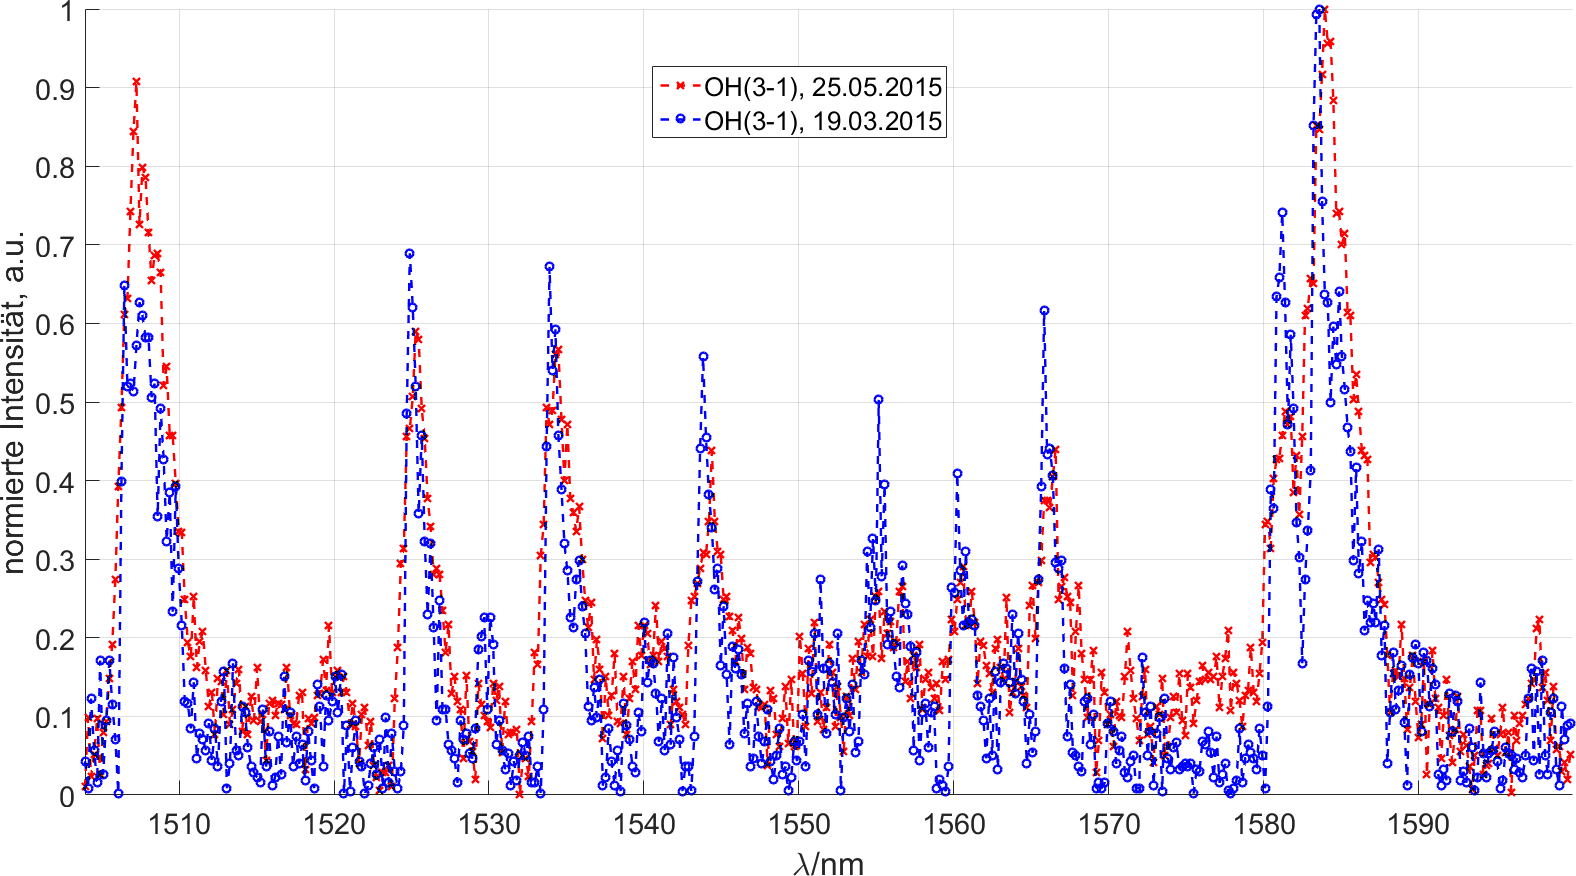
\includegraphics[width=0.9\textwidth]{spektr_unsmooth.png}
		\caption{Betrag der Differenz aus gemessenem Spektrum und Dunkelstrom-Intensität $|I-I\ix{0}|$. Gezeigt sind Verläufe vom 25.05. und 19.03.2015.}
		\label{img:spektr1}
	\end{figure}
	
	Die \autoref{img:spektr2} zeigt die geglätteten, normierten Messwerte. Insbesondere die Struktur der $P\ix{1}(j)$- und $P\ix{2}(i)$-Peaks, welche nur durch das ungepaarte Elektron unterschieden werden, kann sehr gut beobachtet werden. Jedoch ist durch die Glättung natürlich eine gewisse Einbuße an Peak-Höhe zu verzeichnen, was für die Betrachtung der Rotationsbande aber keine Rolle spielt.\\
	Links und rechts im Spektrum sind deutlich die Maxima der ersten Q-Zweige $\fett{OH}(4-2)$ bzw. $\fett{OH}(3-1)$ zu sehen. Zwischen den hier betrachteten P-Zweigen und dem rechten Rand finden sich die Flachen Linien des R-Zweiges $\fett{OH}(4-2)$. Sogar die Emissionslinie für $P\ix{1}(1)$ kann um $\unit[1600]{nm}$ beobachtet werden.
	
	\begin{figure}[h]
		\centering
		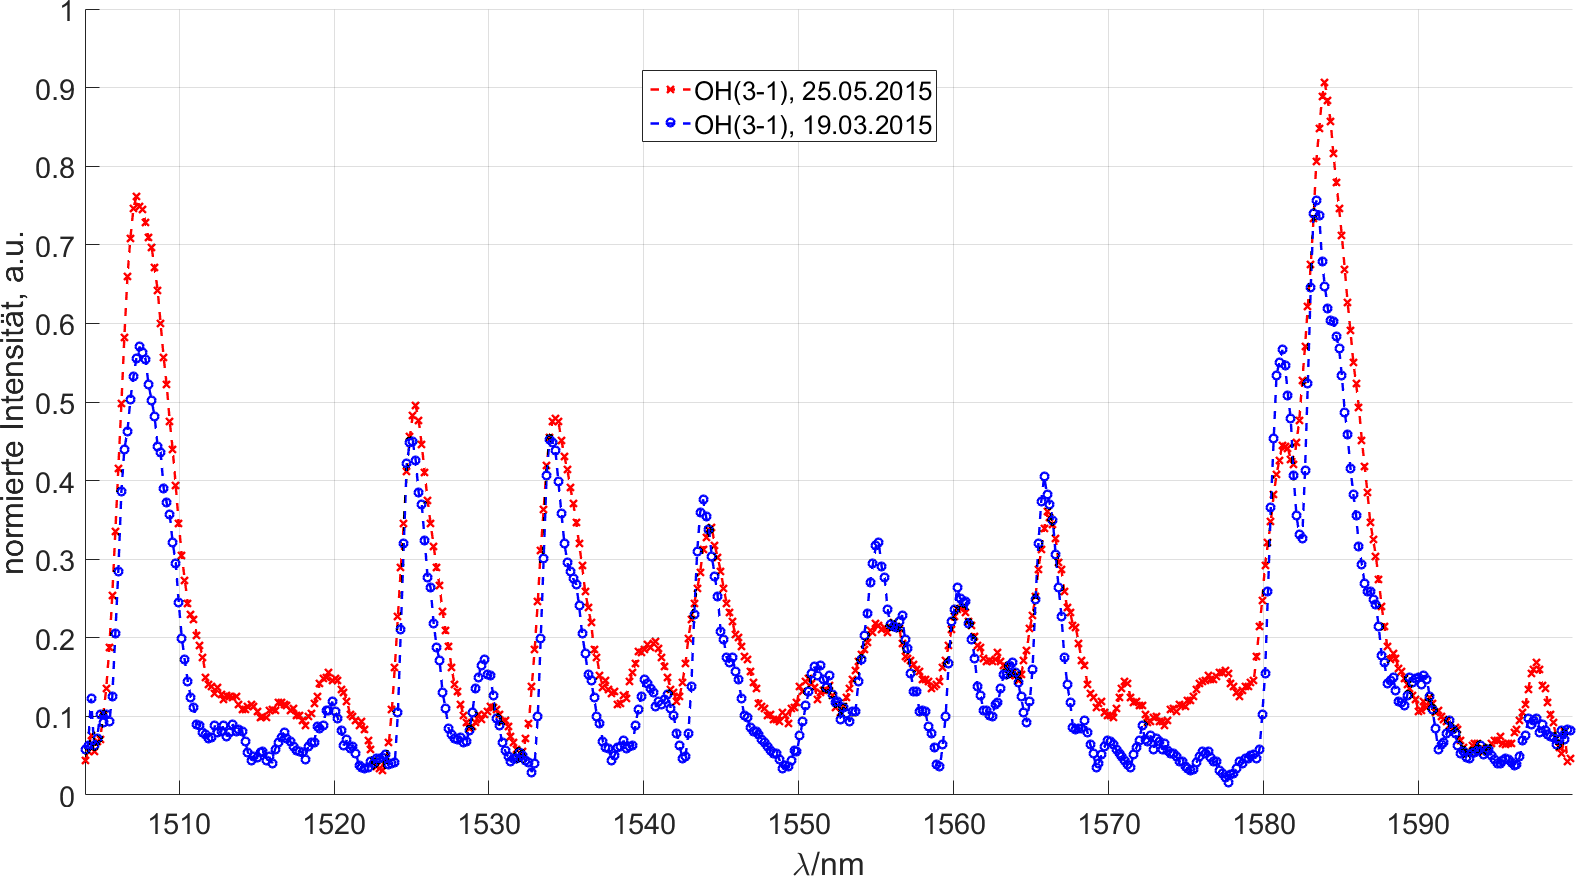
\includegraphics[width=0.9\textwidth]{spektr_smooth.png}
		\caption{Gleiche Daten wie in \autoref{img:spektr1} (Spektrum A, Spektrum B). Hier mit Hilfe einer polynomischen Glättung, maximal der Ordnung 7 verbessert. Der Zusammenhang kommt auf \autoref{eq:glatt}}
		\label{img:spektr2}
	\end{figure}
	
	\begin{table}[h]
		\centering
		\begin{tabular}{c|c|c|c}
			Peaknummer & $\lambda/\unit[\tenpo{3}]{nm}$, aus \cite{EMAUGreifswaldOHRot} & $\lambda/\unit[\tenpo{3}]{nm}$, A & $\lambda/\unit[\tenpo{3}]{nm}$, B\\
			\hline $P\ix{1}(2)$ & 1,524 & 1,526 & 1,525 \\
			\hline $P\ix{1}(3)$ & 1,533 & 1,535 & 1,534 \\
			\hline $P\ix{1}(4)$ & 1,543 & 1,545 & 1,544
		\end{tabular}
		\caption{Wellenlängen der Peaks $P\ix{1}(2-4)$ im Vergleich zum Literaturwert aus \cite{EMAUGreifswaldOHRot}. Außerdem Gegenüberstellung der Werte aus den Intensitäten zum Spektrum A und B.}
		\label{tab:wellen}
	\end{table}
	
	Die Positionen der Peaks $P\ix{1}(j)$ der Rotationsübergänge sind in \autoref{tab:wellen} aufgeführt. Deren Intensitäten - ohne Normierung und Glättung, nur nach Korrektur mit Dunkelströmen - finden sich in \autoref{tab:intens}.
	
	\begin{table}[h]
		\centering
		\begin{tabular}{c|c|c}
			Peaknummer & $|I-I\ix{0}|/\tenpo{2}$, zu A & $|I-I\ix{0}|/\tenpo{2}$, zu B\\
			\hline $P\ix{1}(2)$ & 2,993 & 1,995 \\
			\hline $P\ix{1}(3)$ & 2,873 & 1,945 \\
			\hline $P\ix{1}(4)$ & 2,223 & 1,615
		\end{tabular}
		\caption{Höhen der Peaks $P\ix{1}(2-4)$ an den Positionen aus \autoref{tab:wellen}. Gegenüberstellung von Spektrum A und B. Diese Werte sind für die Auswertung mit der linearen Regression aus \autoref{eq:linreg} wichtig.}
		\label{tab:intens}
	\end{table}
	
	\begin{figure}[h]
		\centering
		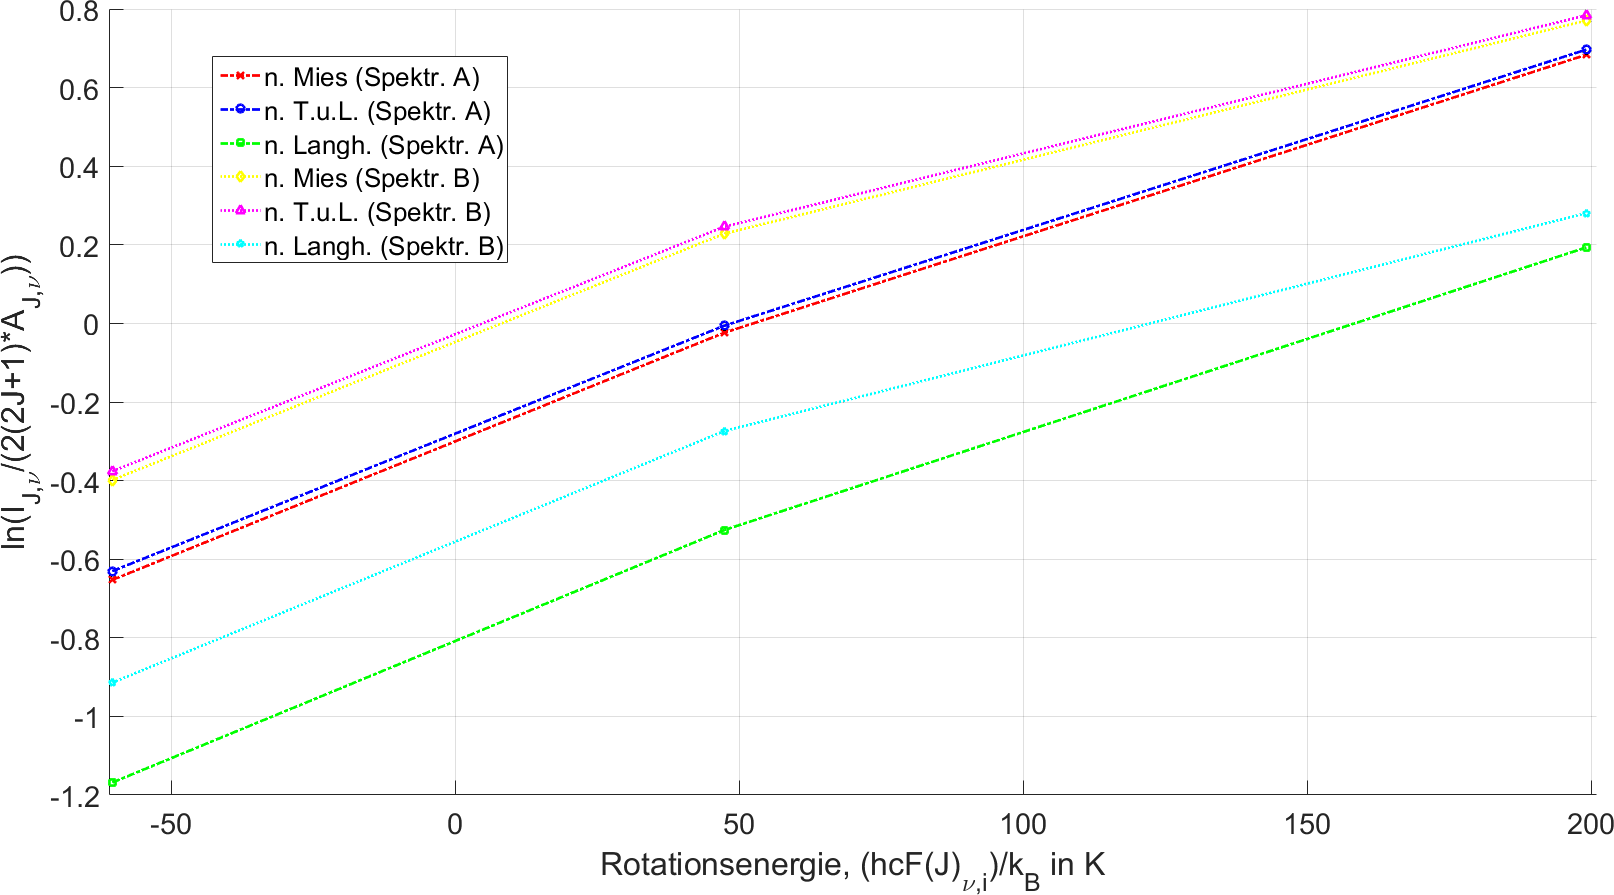
\includegraphics[width=0.9\textwidth]{linear_reg.png}
		\caption{Lineare Regression über die Rotationsenergie und Daten aus \autoref{tab:intens}.}
		\label{img:regress}
	\end{figure}
	
	Schließlich wurde aus den gemessenen Daten die Rotationstemperatur bestimmt. Dabei gehen die verschiedenen, theoretisch begründeten Einsteinkoeffizienten $A(\lambda\rightarrow\lambda^\prime)$ ein (siehe Mies, Langhoff usw.). Jeweils für Spektrum A und B wurde die lineare Regression nach dem Vorbild aus \autoref{eq:linreg} für 3 verschiedene Übergangswahrscheinlichkeiten durchgeführt. Das graphische Resultat findet sich in \autoref{img:regress}, die daraus erhaltenen Temperaturen in \autoref{tab:trot}.
	
	\begin{table}[h]
		\centering
		\begin{tabular}{c|c|c}
			Einsteinkoeffizienten, aus \cite{EMAUGreifswaldOHRot} & $T\ix{rot}/\unit{K}$, zu A & $T\ix{rot}/\unit{K}$, zu B\\
			\hline Mies (1947) & 347,98 & 241,75 \\
			\hline Turnbull u. Lowe (1989) & 342,44 & 239,06 \\
			\hline Langhoff (1986) & 1120,1 & 463,93
		\end{tabular}
		\caption{Rotationstemperaturen nach \autoref{eq:linreg}. Die Fehler nach Gauß sind in \autoref{eq:err} angegeben. Für die Intensität wurde das Dunkelstromkorrigierte Spektrum $|I-I\ix{0}|$ benutzt.}
		\label{tab:trot}
	\end{table}
	
	\subsection{Fehlerrechnung}
	
	%				\begin{figure}
	%					\centering
	%					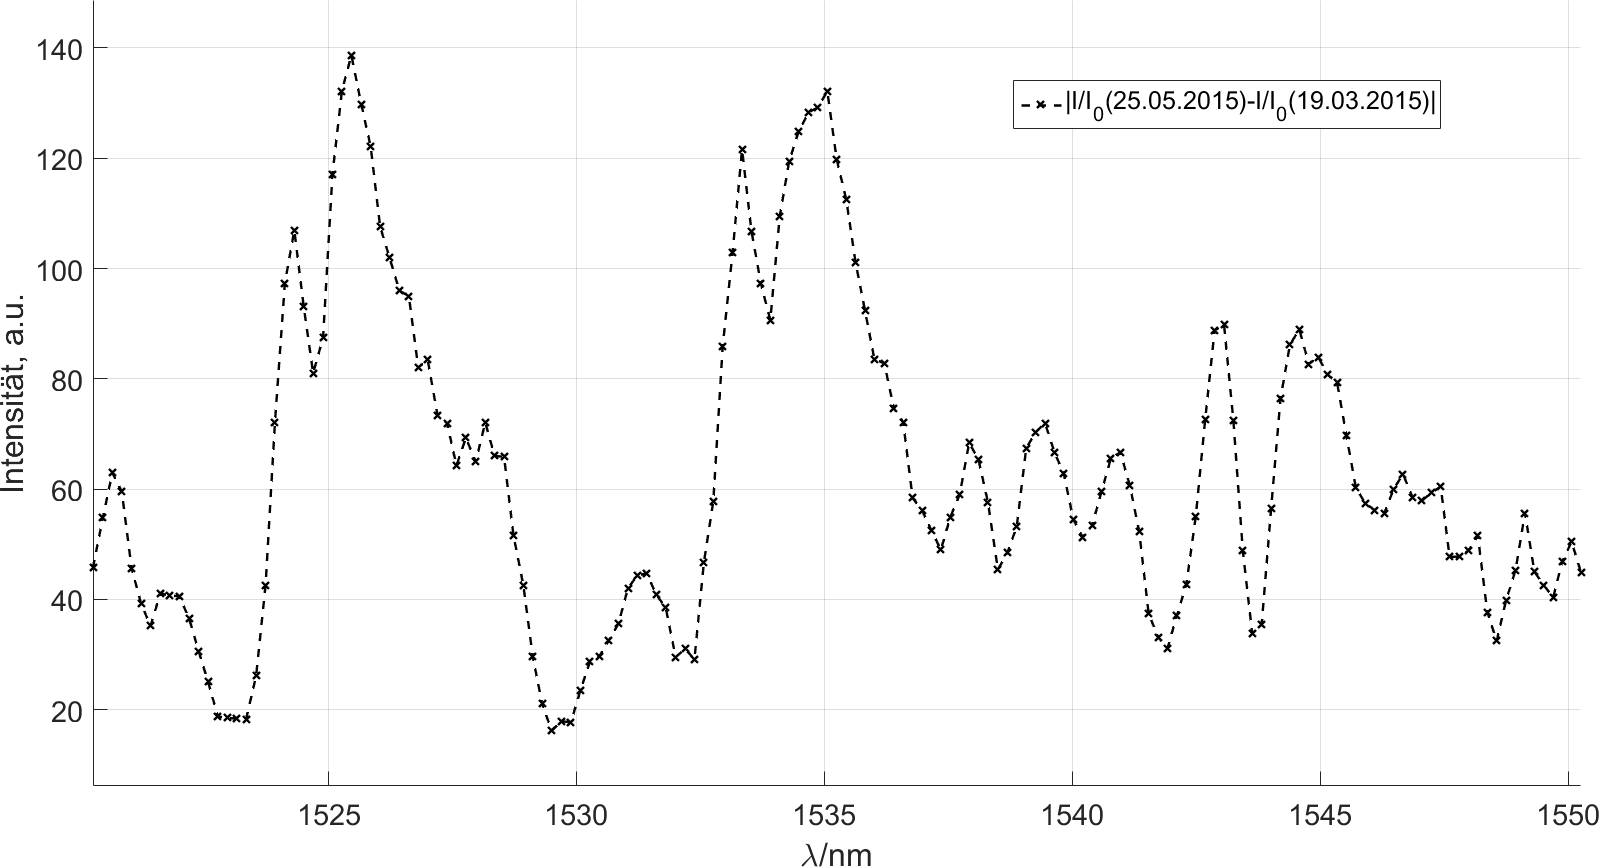
\includegraphics[width=0.9\textwidth]{differenz.png}
	%					\caption{Differenz aus Spektrum A und B. Ebenso wie \autoref{img:spektr2} über Polynome geglättet.}
	%					\label{img:diff}
	%				\end{figure}
	
	Die in \autoref{tab:trot} berechneten Temperaturen verschiedener Theorien zeigen bereits, welchen Effekt die unterschiedlichen Annahmen über die quantenmechanischen Prozesse der Molekül-Übergänge haben können. Insbesondere die Berechnungen nach Langhoff et. al. weichen sehr stark von den übrigen 2 Werten ab.\\
	Über die Fehlerrechnung nach \tilt{Gauß} aus \autoref{eq:gauss} kann zudem ein weiteres Maß für den Fehler angegeben werden. Dieser ergibt sich, für Spektrum A und B nach Bestimmung der Standardabweichung (nach Maßgabe aus \cite{EMAUGreifswaldOHRotat}), in \autoref{eq:err}. Die Fortpflanzung des Fehlers $\Delta I_{\nu,i,J}$ über die lineare Regression der \autoref{eq:linreg} in den Rotationstemperaturen gibt \autoref{eq:err2} wieder. Für beide Fälle - Spektrum A und B und für die \tilt{gauß'sche} Fehlerfortpflanzung - wurden die Koeffizienten nach Mies benutzt.
	
	\begin{align}
	T\ix{rot}\left(I,\nu,i,J\right)\propto-&\frac{hcF\left(J,\nu,i\right)}{k\ix{B}}\ln\left(\frac{I\left(\nu,i,J\leftarrow\nu\prime,i\prime,J\prime\right)}{2\left(2J+1\right)A\left(\nu,i,J\rightarrow\nu\prime,i\prime,J\prime\right)}\right)^{-1} \\
	\Delta& T\ix{rot}\approx\sqrt{\left(\frac{\diff T\ix{rot}}{\diff I_{\nu,i,J}}\right)^2\cdot\left(\Delta I_{\nu,i,J}\right)^2} \label{eq:gauss}
	\end{align}
	
	\begin{align}
	\text{nach Mies:} \quad &T\ix{rot,A}=\left(347,98\pm 0,0424(11)\right)\unit{K} \label{eq:err}\\
	&T\ix{rot,B}=\left(241,75\pm 0,223(22)\right)\unit{K} \nonumber
	\end{align}
	
	\begin{align}
	\text{nach Mies:} \quad &T^{(A)}\ix{rot,true}\in\left[347,67(03)\unit{K},348,29(02)\unit{K}\right]  \label{eq:err2}\\
	&T^{(B)}\ix{rot,true}\in\left[241,57(63)\unit{K},241,92(90)\unit{K}\right] \nonumber
	\end{align}
	
	\newpage
	\section{Anhang}
	
	\bibliography{all.bib}
	\bibliographystyle{unsrt}
	
\end{document}